\section{Approach}
 This R\&D will focus on designing and developing a visual servoing controller that can manipulate static and dynamic objects. This task is decomposed into simple and achievable
tasks below
\begin{itemize}
\item Survey on the state of the art strategies of visual controllers and critically assess them.
\item Generalize features for all the graspable objects with respect to youBot gripper. Line features will be chosen in the beginning stage to simplify 
visual processing.
\item Design and develop a simple visual servo controller with restricted degrees of control in base and arm to manipulate static objects.
\item Extend the controller to control all joints and encode joint limits, obstacle avoidance, occlusion and visibility constraints.
\item Extend the controller to manipulate dynamic objects.
\end{itemize}
\subsection{Task Specification}
\paragraph{Visual Control System}
The system requires an appropriate number and type of cameras mounted over strategic positions to track the object or visually guide the robot in positioning the base. The main
focus of out task is to achieve successful manipulation, which gives us a bit of idea to choose camera positions.In RoboCup@Work scenario, or any other new environment, it is
always preferred to have a camera over the arm which is positioned in such a way to monitor the object with wide visibility. Also, there are various camera types which has a 
potential impact on the type of features it can perceive. An appropriate definition of features with respect to ability of gripper to do successful grasping will help in deciding the right camera. In such systems, there is a possibility 
that the camera can lose the target due to the motion of base around the object to afford arm reachability. In such cases, we need another camera to monitor the state of the 
object which can guide the robot. 
\paragraph{Implementation Details}
 \begin{itemize}
\item The implementation will start with an idea of detecting two dimensional line features which can generalize all the proposed graspable objects. A primitive level visual control which can handle only four specific joints of the base and arm is developed. In control terms, a feature Jacobian of dimension four will be built to 
control the velocity of limited joints. This implementation is done to find out issues in features and upcoming control problems.
\begin{figure}[here]
 \vspace{2 mm}
  \centerline {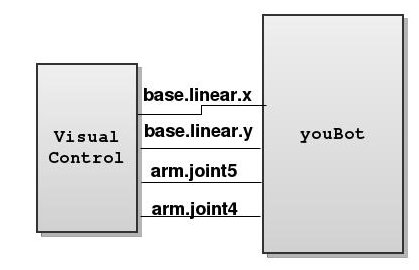
\includegraphics[scale=0.44]{images/vs_primitive}}
  \caption{Primitive Visual Control}
 \vspace{2 mm}
\label{fig:primviscont}
\end{figure}
\newline
The figure \ref{fig:primviscont} shows an overview of the controller. Pre-grasp arm joint positions are chosen for other joints to ensure the object in the visual field 
of the camera.

\item The development will target on mapping feature error to all the joints of the robot to have a whole body control. A rough overview of the system is below.
\begin{figure}[there]
 \vspace{2 mm}
  \centerline {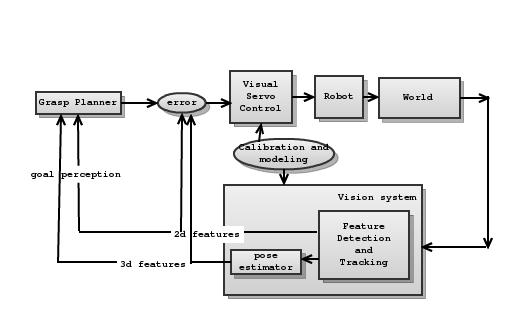
\includegraphics[scale=0.6]{images/vs_youbot}}
  \caption{Visual Control Overview}
 \vspace{2 mm}
 \label{fig:viscont}
\end{figure}
\end{itemize}

\section{Evaluation Stategy}
Evaluation of the developed algorithm is to be done on the proposed objects which affords to grasping ability of the KUKA youbot gripper and has significant line features. The 
joint velocity components, evolution of errors, the number of iterations and other necessary parameters will be monitored. Stability analysis of the
control algorithm is performed to evaluate the performance of the algorithm.
\paragraph{Stability Analysis of Closed Loop Control}
Lyapunov analysis will be used to determine the stability of the control algorithm\cite{Hutchinson2006}. The Lyapunov function $L =  1/2\parallel  e  \big(t\big) \parallel ^{2}$
will be used to analyse the global and local assymptotic stability of the system by testing on various task constraints listed below.
\begin{itemize}
\item Initial camera positions by varying along one degree of freedom or multiple degree of freedom as done in \cite{jagersand1997experimental}. Various camera positions
enable to evaluate the algorithms under local minima.
\item Initial robot base positions based on how close it is with respect to the platforms and other obstacles. 
\end{itemize}
The above list will get updated in the course of the project to measure the performance effectively.








